\documentclass[12pt,a4paper]{article}
\usepackage[utf8]{inputenc}
\usepackage[T1]{fontenc}
\usepackage[english]{babel}
\usepackage{graphicx}
\usepackage[left=2.5cm,right=2.5cm,top=3cm,bottom=3cm]{geometry}
\usepackage{hyperref}
\usepackage{csquotes}
\usepackage{natbib}
\usepackage{doi}
% --- packages added for this report ---
\usepackage{booktabs}      % nice tables
\usepackage{xcolor}
\usepackage{listings}      % code / triple listings
\usepackage{tikz}          % architecture diagram (no external image needed)
\usetikzlibrary{arrows.meta,positioning,shapes.geometric}
\usepackage{placeins}      % \FloatBarrier: keep floats from drifting into later text

% listing style for RDF triples / JSON / code
\lstset{
  basicstyle=\ttfamily\small,
  breaklines=true,
  frame=single,
  columns=fullflexible,
  keepspaces=true,
  showstringspaces=false,
  xleftmargin=1em,
}

%opening
\title{A Semantic Knowledge-Graph Expert System \\ for Wine-Component Recommendation}
\author{Myron Melnyk}
\date{11 July 2026}

\begin{document}

	\maketitle

	\section*{Introduction}
	% (about 0.5 pages)
	A wine is described by measurable \textbf{components}, such as alcohol, acidity,
	or sugar. In this project we do not use the exact measured numbers. Instead, for
	each component we only say how big it is: its \textbf{level} is \emph{low},
	\emph{middle}, or \emph{high}. For example, a wine can have \emph{high alcohol},
	\emph{low sugar}, or \emph{middle acidity}. We call one such pair -- a component
	together with its level -- a \emph{component state} (for example
	\texttt{high\_alcohol}). Our system takes one component state chosen by the user
	(for example \emph{low chlorides}) and suggests other component states that
	usually appear together with it in the best wines. For each suggestion it also
	shows \emph{why} it was chosen.

	This is a \emph{knowledge representation} problem, not only a statistics problem.
	A normal machine-learning model could guess a quality score, but it could not
	tell the user which things go together, or explain why. We want knowledge that is
	written down clearly, that a person can read, and that the program can reason
	about and explain. So we store the component states and the links between them as
	an explicit graph.

	We answer three questions:
	\begin{itemize}
		\item \textbf{RQ1.} How can we turn the exact measured numbers into simple
		concepts such as \emph{high alcohol}?
		\item \textbf{RQ2.} Which component states appear together in the best wines,
		and how can we store this knowledge as a graph?
		\item \textbf{RQ3.} Besides directly linked components, can the system also
		recommend a component through a \emph{shared connection} -- a middle
		component that both are linked to?
	\end{itemize}

	\section*{Background and related work}
	% (about 1 page)
	\paragraph{Background.}
	To understand this report we need three simple ideas from knowledge
	representation:
	\begin{itemize}
		\item \textbf{Semantic network} (also called a \emph{knowledge graph}) --
		knowledge stored as \emph{nodes} joined by \emph{links}. A node is a thing or
		an idea (for us, a component state such as \texttt{high\_alcohol}); a link says
		how two nodes are related.
		\item \textbf{Ontology} -- the same idea, but with strict rules about which
		kinds of nodes and links are allowed.
		\item \textbf{RDF triple} -- one fact written as three parts,
		\emph{subject -- relation -- object}, for example
		``\texttt{high\_alcohol} -- hasLevel -- high''.
	\end{itemize}
	We use a \textbf{semantic network} (the view taught in the course lectures
	\citep{khalid2026semnet}). The other two matter because our graph can also be
	written as RDF triples, and could later grow into a full ontology.

	\paragraph{Related work.}
	Our method -- building a network from how often items appear together -- is the
	standard approach in \emph{semantic network analysis} of \emph{verbal fluency}
	data \citep{christensen2023semna}. In the classic task, people name as many
	animals as they can; a network is then built from which animals are named
	together across many people, so that animals that often co-occur become
	connected. This is exactly the method introduced in our course
	\citep{khalid2026semnet}, where we built such a co-occurrence network from an
	animal-naming dataset. Our project applies the same idea to a different domain:
	instead of animals named by a person, our items are wine component states, and
	instead of one person's list we use one wine's set of components. The wine data
	comes from the UCI Wine Quality dataset \citep{wine_quality_186}.

	\section*{Knowledge source and representation}
	% (about 1 page)
	\paragraph{Source.} The knowledge is derived from the UCI \emph{Wine Quality}
	dataset \citep{wine_quality_186} (\url{https://doi.org/10.24432/C56S3T}). It
	contains Portuguese \emph{Vinho Verde} samples described by 11 physicochemical
	features (fixed acidity, volatile acidity, citric acid, residual sugar,
	chlorides, free sulfur dioxide, total sulfur dioxide, density, pH, sulphates,
	alcohol) plus an expert \emph{quality} score. Red and white wines are provided
	as separate files and modelled separately.

	\paragraph{From numbers to concepts (RQ1).} Raw measurements are not knowledge;
	they become knowledge only once they are given meaning. For each feature we take
	its observed range $[\min,\max]$, split it into three equal-width intervals, and
	map every value to a qualitative \emph{level} concept -- \emph{low}, \emph{middle},
	or \emph{high}. A measurement such as ``alcohol $= 12.8$'' becomes the symbolic
	concept \texttt{high\_alcohol}. This discretisation is the bridge from data to
	knowledge and is what makes the rest of the system symbolic and explainable.

	\paragraph{Representation model (RQ2).} We represent the knowledge as a
	\textbf{typed semantic network}. Its schema is small and explicit:

	\begin{table}[h]
	\centering
	\begin{tabular}{@{}lp{9.5cm}@{}}
	\toprule
	\textbf{Concept / class} & \textbf{Meaning} \\
	\midrule
	\texttt{Component}      & a physicochemical property, e.g. \emph{alcohol}, \emph{chlorides} \\
	\texttt{Level}          & a qualitative value: \emph{low}, \emph{middle}, \emph{high} \\
	\texttt{ComponentState} & a component observed at a level, e.g. \texttt{high\_alcohol} \\
	\texttt{Quality}        & the wine-quality class used as context (the best wines) \\
	\texttt{Wine}           & the wine type providing context: red or white \\
	\bottomrule
	\end{tabular}
	\caption{The concepts (classes) in the model.}
	\label{tab:classes}
	\end{table}

	\begin{table}[h]
	\centering
	\begin{tabular}{@{}lll@{}}
	\toprule
	\textbf{Relation} & \textbf{Domain $\rightarrow$ Range} & \textbf{Meaning} \\
	\midrule
	\texttt{hasComponent} & ComponentState $\rightarrow$ Component & which component \\
	\texttt{hasLevel}     & ComponentState $\rightarrow$ Level     & at which level \\
	\texttt{coOccursWith} & ComponentState $\leftrightarrow$ ComponentState & jointly present in the best wines (weighted) \\
	\bottomrule
	\end{tabular}
	\caption{The relations (links) in the model.}
	\label{tab:relations}
	\end{table}

	Each node in the knowledge base is now \emph{self-describing}: it stores its
	type, component and level. Each edge is a \emph{typed} \texttt{coOccursWith}
	relation whose \texttt{weight} records how many of the best wines contain both
	states. The same knowledge is expressible as RDF triples (RQ2), which we use as
	the conceptual reading of the graph:

	\FloatBarrier
\begin{lstlisting}[caption={One node and one link, as triples and as stored JSON.},captionpos=b,label={lst:triples}]
# --- as RDF triples (conceptual reading) ---
:high_alcohol   a               :ComponentState .
:high_alcohol   :hasComponent   :alcohol .
:high_alcohol   :hasLevel       :High .
:low_chlorides  :coOccursWith   :low_total_sulfur_dioxide .   # weight 18 (best red wines)

# --- as actually stored in knowledge_base.json ---
{ "id": "low_chlorides", "type": "ComponentState",
  "component": "chlorides", "level": "low" }
{ "source": "low_chlorides", "target": "low_total_sulfur_dioxide",
  "weight": "18", "relation": "coOccursWith" }
\end{lstlisting}

	This representation is suitable because the concepts are symbolic and
	inspectable, the relations are typed and therefore machine-interpretable, and the
	graph structure directly supports the traversal-based inference described below.

	\section*{System architecture}
	% (about 0.5 to 1 pages)
	The system has three modules (Fig.~\ref{fig:arch}): a Python
	\emph{knowledge-acquisition} pipeline that builds the knowledge base; the
	\emph{knowledge base} itself (\texttt{knowledge\_base.json}); and a Next.js
	application containing the \emph{inference engine} and the \emph{user interface}.
	The pipeline is the single source of truth; the application only reads the
	knowledge base and never mutates it.

	\begin{figure}[h]
	\centering
	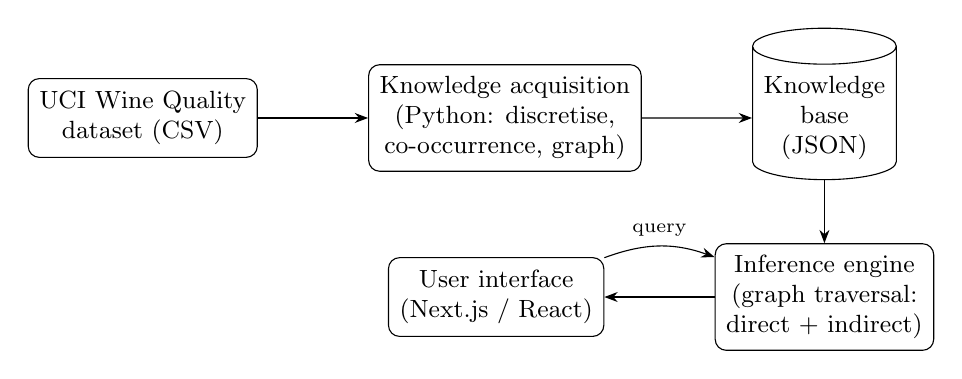
\begin{tikzpicture}[
		node distance=8mm and 14mm,
		box/.style={draw,rounded corners,align=center,minimum height=10mm,inner sep=4pt,font=\small},
		db/.style={draw,cylinder,shape border rotate=90,aspect=0.25,align=center,inner sep=4pt,font=\small},
		>={Stealth[]}
	]
		\node[box] (data) {UCI Wine Quality\\dataset (CSV)};
		\node[box,right=of data] (build) {Knowledge acquisition\\(Python: discretise,\\co-occurrence, graph)};
		\node[db,right=of build] (kb) {Knowledge\\base\\(JSON)};
		\node[box,below=of kb] (engine) {Inference engine\\(graph traversal:\\direct + indirect)};
		\node[box,left=of engine] (ui) {User interface\\(Next.js / React)};
		\draw[->] (data) -- (build);
		\draw[->] (build) -- (kb);
		\draw[->] (kb) -- (engine);
		\draw[->] (engine) -- (ui);
		\draw[->] (ui) to[bend left=20] node[midway,above,font=\scriptsize] {query} (engine);
	\end{tikzpicture}
	\caption{The three parts of the system and how the data flows between them.}
	\label{fig:arch}
	\end{figure}

	\textbf{Knowledge acquisition} discretises the measurements, keeps only the
	best wines, counts co-occurrences and emits the typed graph.
	\textbf{The knowledge base} stores the two typed semantic networks (red, white)
	plus the list of all component states.
	\textbf{The inference engine} (\texttt{WineRecommendationService}) answers
	recommendation queries by traversing the graph.
	\textbf{The user interface} lets the user pick a component state and shows the
	ranked recommendations with their explanations.

	\section*{Implementation}
	% (about 2 to 3 pages)
	\subsection*{Building the knowledge base}
	The pipeline (\texttt{data-builder/}, Python with \texttt{pandas} and
	\texttt{networkx}) proceeds as follows:
	\begin{enumerate}
		\item \textbf{Discretise.} Each numeric feature is binned into
		\emph{low}/\emph{middle}/\emph{high} by equal-width intervals over its
		observed range, producing a \texttt{ComponentState} label per cell.
		\item \textbf{Select the best wines.} Only rows with the top quality score
		(\texttt{quality == 8}) are kept, so the knowledge describes what
		characterises \emph{excellent} wine.
		\item \textbf{Count co-occurrences.} For those wines we count how often each
		pair of component states appears together, giving a weighted association.
		\item \textbf{Build the typed graph.} Pairs whose count exceeds a threshold
		become \texttt{coOccursWith} edges; isolated nodes are removed; each node is
		annotated with its \texttt{type}, \texttt{component} and \texttt{level}.
		\item \textbf{Serialise.} The two graphs are written to
		\texttt{knowledge\_base.json}.
	\end{enumerate}
	The threshold is set per wine type because the number of top-quality samples
	differs sharply: it is $6$ for red and $120$ for white. As a consequence the
	maximum edge weight roughly equals the number of best wines available
	($\approx 18$ for red, $\approx 175$ for white); the threshold keeps only
	associations that are frequent \emph{relative} to that pool.

	\subsection*{Reasoning over the knowledge (RQ3)}
	Given a query component state, the engine
	(\texttt{app/utils/recommendation-engine.ts}) performs graph traversal:
	\begin{itemize}
		\item \textbf{Direct inference.} Every \texttt{coOccursWith} neighbour of the
		query is a candidate. Its score is the edge weight normalised to the strongest
		edge in the graph: $\mathrm{score} = \mathrm{round}(100 \cdot w / w_{\max})$.
		\item \textbf{Indirect inference (new knowledge).} If the query $X$ co-occurs
		with $Y$ and $Y$ co-occurs with $Z$, the engine \emph{infers} an association
		$X\!-\!Z$ that is \textbf{not stored in the knowledge base}, with strength
		$\min(w_{XY}, w_{YZ})$ and an explanation recording the intermediate node $Y$
		(see the diagram below). This is the step where the system produces
		knowledge beyond the stored facts.
		\item \textbf{Consistency filter.} The chosen component is never recommended
		back at another level: if the query is \texttt{low\_chlorides}, the results
		never contain \texttt{middle\_chlorides} or \texttt{high\_chlorides}. This
		avoids telling the user to change the very thing they asked about.
	\end{itemize}
	Candidates are ranked by score, and the best ones are returned. In short, asking
	for a recommendation means asking the graph a simple question: which component
	states are linked to $X$ -- directly, or through one shared middle state -- with
	the strongest links first.

	\subsection*{How the system infers new knowledge}
	\begin{center}
	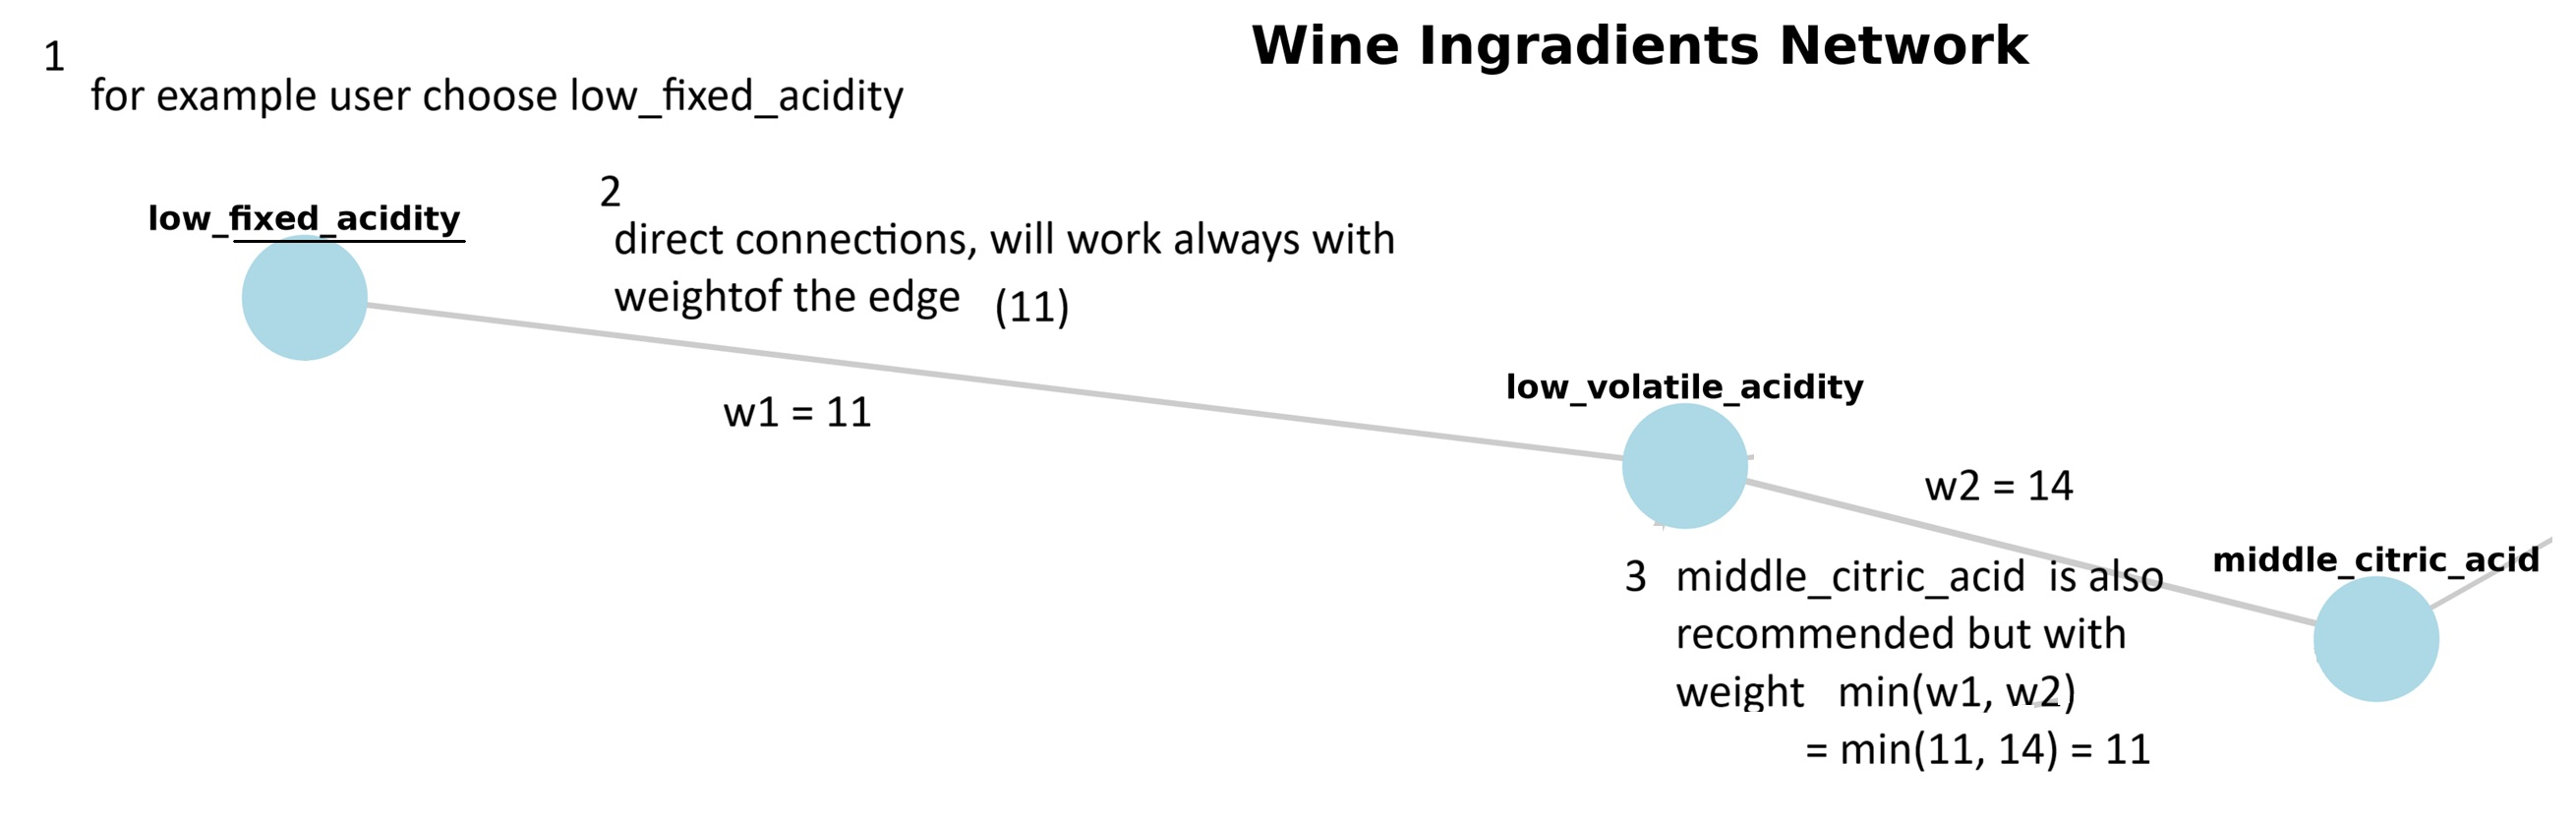
\includegraphics[width=\textwidth]{../imgs/shared_neighbour_concept.jpg}
	\end{center}
	\noindent Here a link that was never stored (\texttt{low\_fixed\_acidity} to
	\texttt{middle\_citric\_acid}) is worked out from two links that were. (Weights
	are illustrative.)

	\subsection*{Tools and interaction}
	The knowledge base is built in Python (\texttt{pandas}, \texttt{networkx},
	\texttt{matplotlib}). The application is built with Next.js~16, React~19 and
	TypeScript; the knowledge base is a plain JSON file loaded at runtime. The user
	selects a component state in the browser and receives the ranked
	recommendations, each labelled as \emph{direct} or \emph{indirect}. For indirect
	ones, it also shows the middle state that connects them -- the reason the
	recommendation was made.

	\section*{Evaluation and discussion}
	% (about 1.5 to 2 pages)
	\subsection*{Knowledge base size}
	Table~\ref{tab:stats} summarises the resulting knowledge base. In total there
	are 33 possible component states (11 components $\times$ 3 levels); the graphs
	retain those that survive the co-occurrence threshold.

	\begin{table}[h]
	\centering
	\begin{tabular}{@{}lcccc@{}}
	\toprule
	\textbf{Graph} & \textbf{Nodes} & \textbf{Edges} & \textbf{Weight range} & \textbf{Threshold} \\
	\midrule
	Red wine   & 14 & 24 & 7--18    & 6   \\
	White wine & 9  & 13 & 128--175 & 120 \\
	\bottomrule
	\end{tabular}
	\caption{Size of the two graphs.}
	\label{tab:stats}
	\end{table}

	Figure~\ref{fig:graphs} shows the two graphs themselves.

	\begin{figure}[ht]
	\centering
	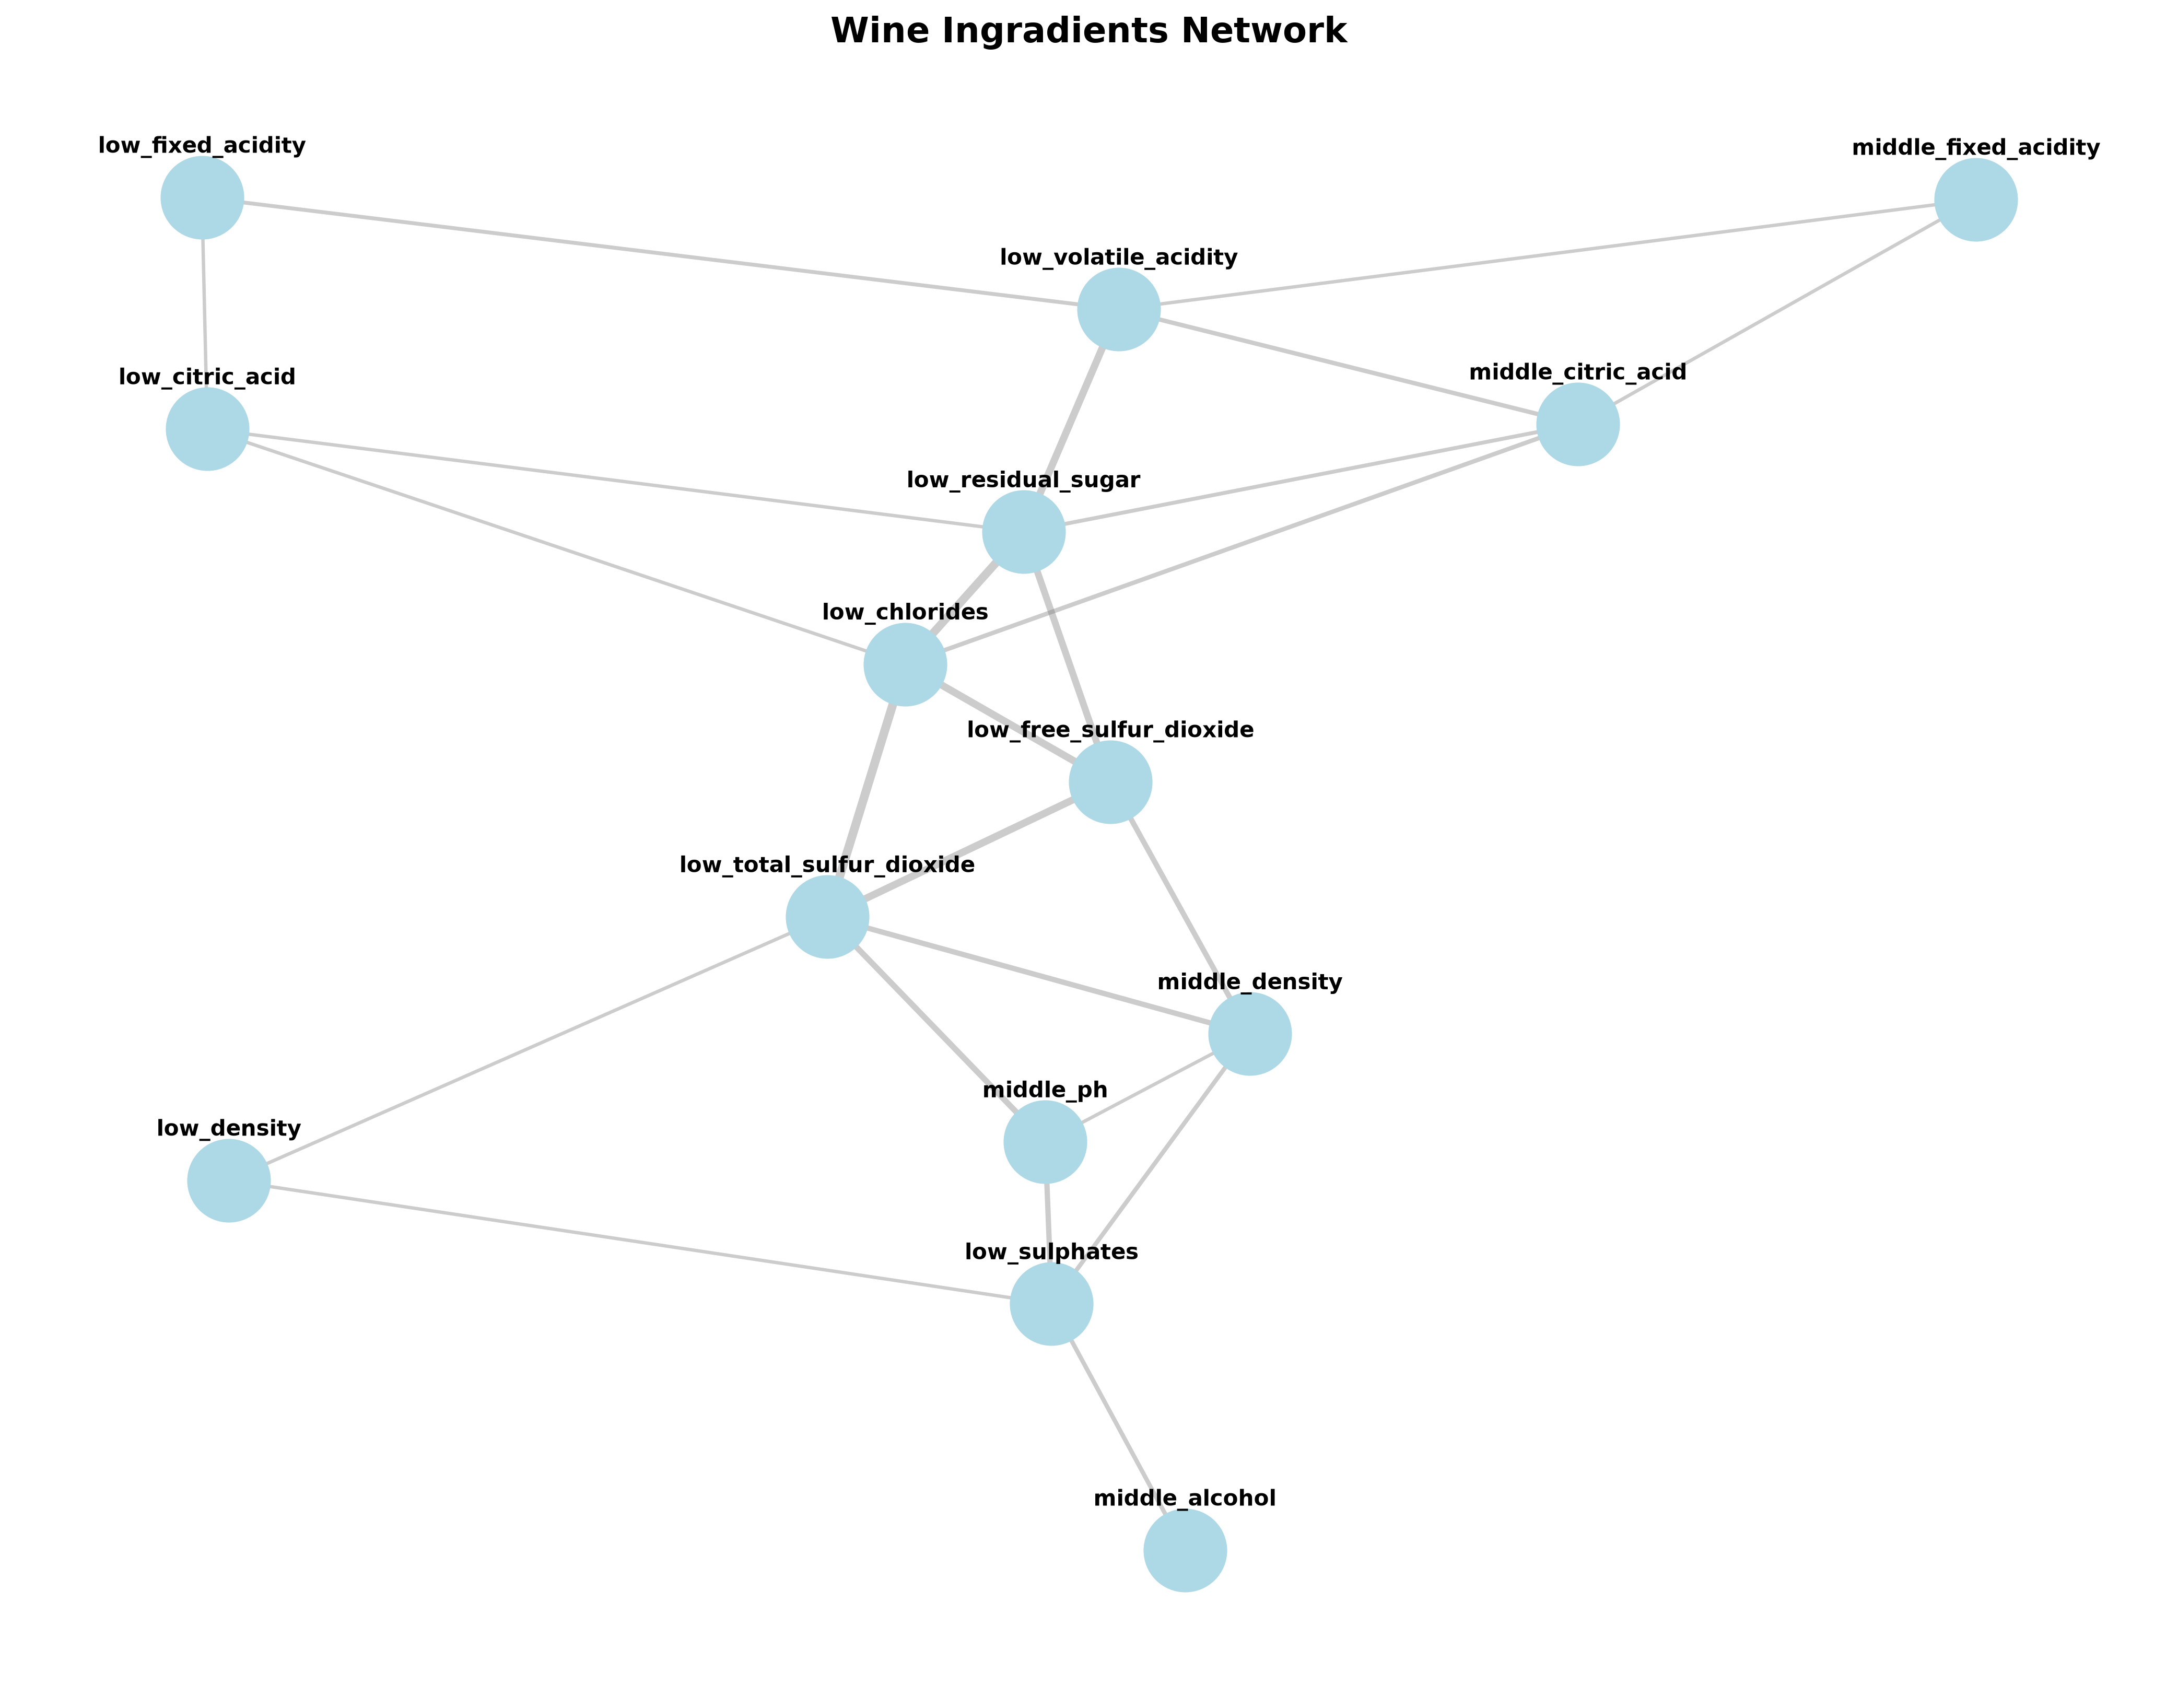
\includegraphics[width=0.49\textwidth]{../imgs/semantic_network_red.png}\hfill
	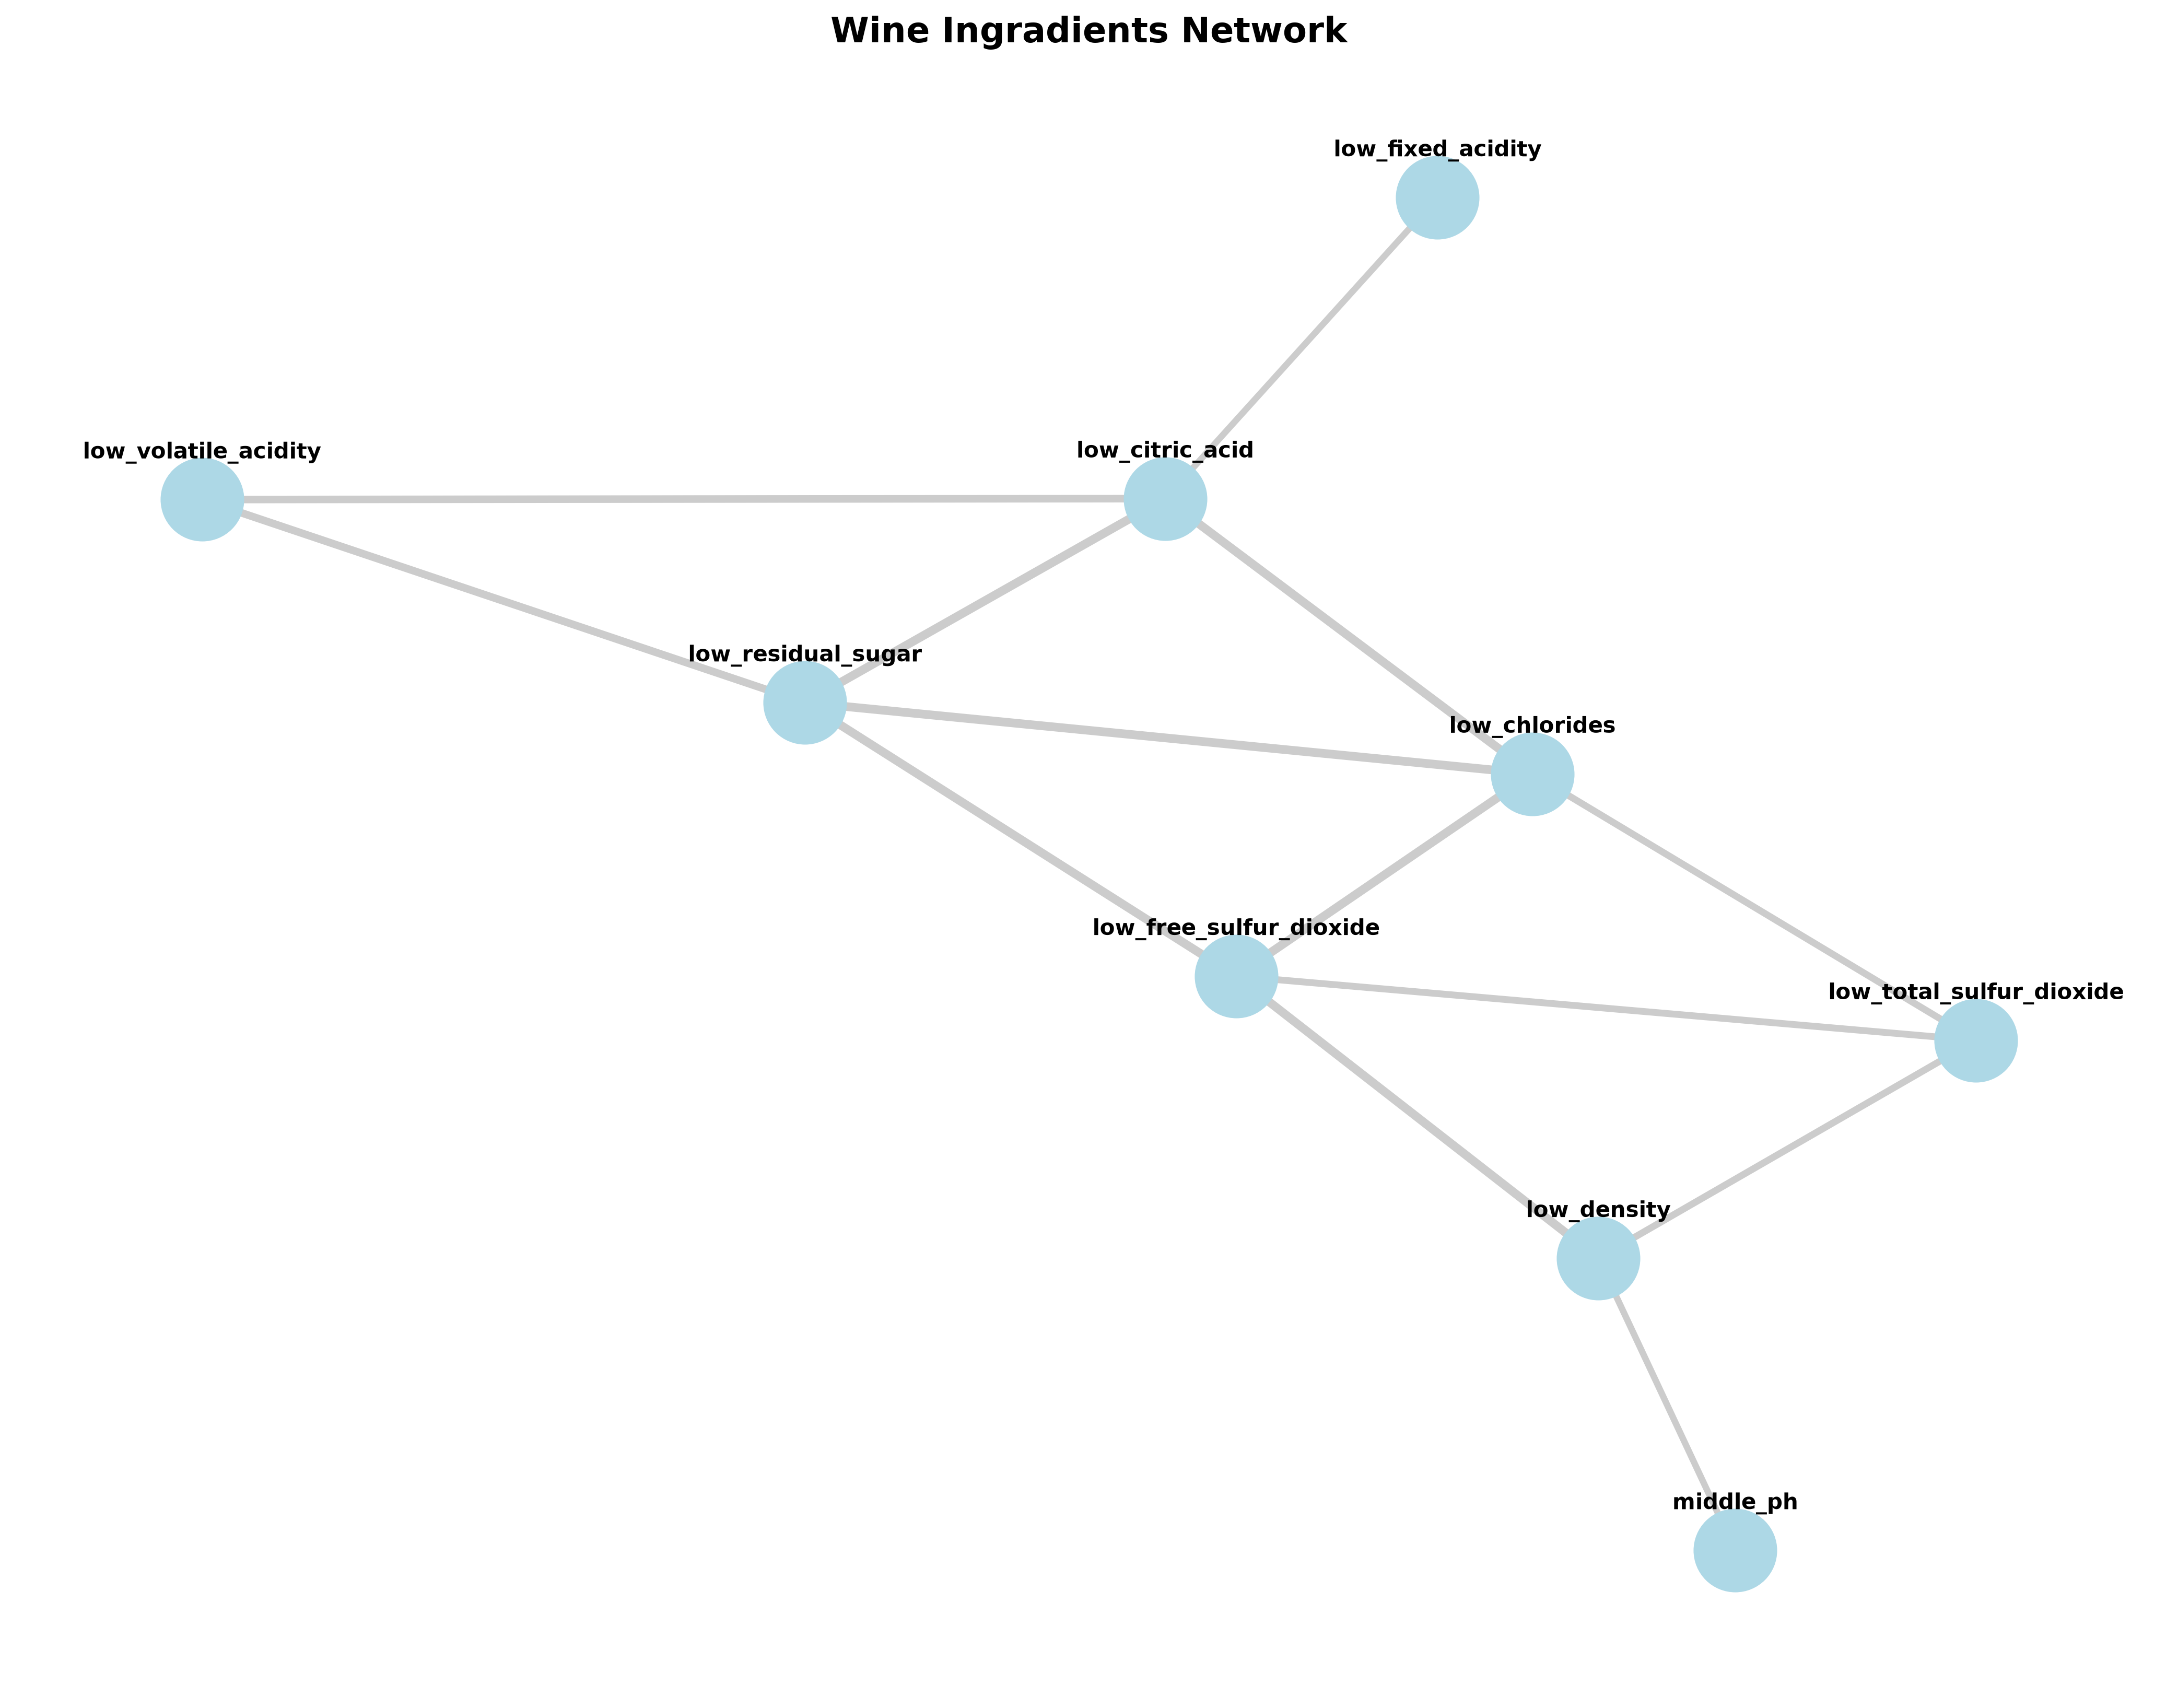
\includegraphics[width=0.49\textwidth]{../imgs/semantic_network_white.png}
	\caption{The two knowledge graphs -- red wine (left, 14 nodes) and white wine
	(right, 9 nodes). Each node is a component state; each link is a
	\texttt{coOccursWith} relation.}
	\label{fig:graphs}
	\end{figure}

	\FloatBarrier
	\subsection*{Worked example: tracing the reasoning}
	We query the red-wine knowledge base for recommendations for
	\texttt{low\_chlorides}. Its stored (direct) \texttt{coOccursWith} neighbours are
	\texttt{low\_total\_sulfur\_dioxide} ($w{=}18$),
	\texttt{low\_residual\_sugar} ($17$),
	\texttt{low\_free\_sulfur\_dioxide} ($15$),
	\texttt{middle\_citric\_acid} ($9$) and
	\texttt{low\_citric\_acid} ($7$). With $w_{\max}=18$, the engine returns the
	ranked list in Table~\ref{tab:trace}.

	\begin{table}[h]
	\centering
	\begin{tabular}{@{}llcl@{}}
	\toprule
	\textbf{Recommended state} & \textbf{Type} & \textbf{Score} & \textbf{Explanation} \\
	\midrule
	\texttt{low\_total\_sulfur\_dioxide} & direct   & 100 & co-occurs directly ($w{=}18$) \\
	\texttt{low\_residual\_sugar}        & direct   & 94  & co-occurs directly ($w{=}17$) \\
	\texttt{low\_free\_sulfur\_dioxide}  & direct   & 83  & co-occurs directly ($w{=}15$) \\
	\texttt{low\_volatile\_acidity}      & indirect & 83  & inferred via \texttt{low\_residual\_sugar} \\
	\texttt{middle\_ph}                  & indirect & 67  & inferred via \texttt{low\_total\_sulfur\_dioxide} \\
	\bottomrule
	\end{tabular}
	\caption{Recommendations for \texttt{low\_chlorides} (red graph). The last two are
	indirect -- found through a shared middle state.}
	\label{tab:trace}
	\end{table}

	Figure~\ref{fig:ui} shows the same query in the web app: choosing
	\texttt{low\_chlorides} on the red-wine graph gives exactly the list in
	Table~\ref{tab:trace}, with both direct recommendations and inferred indirect
	ones.

	\begin{figure}[h]
	\centering
	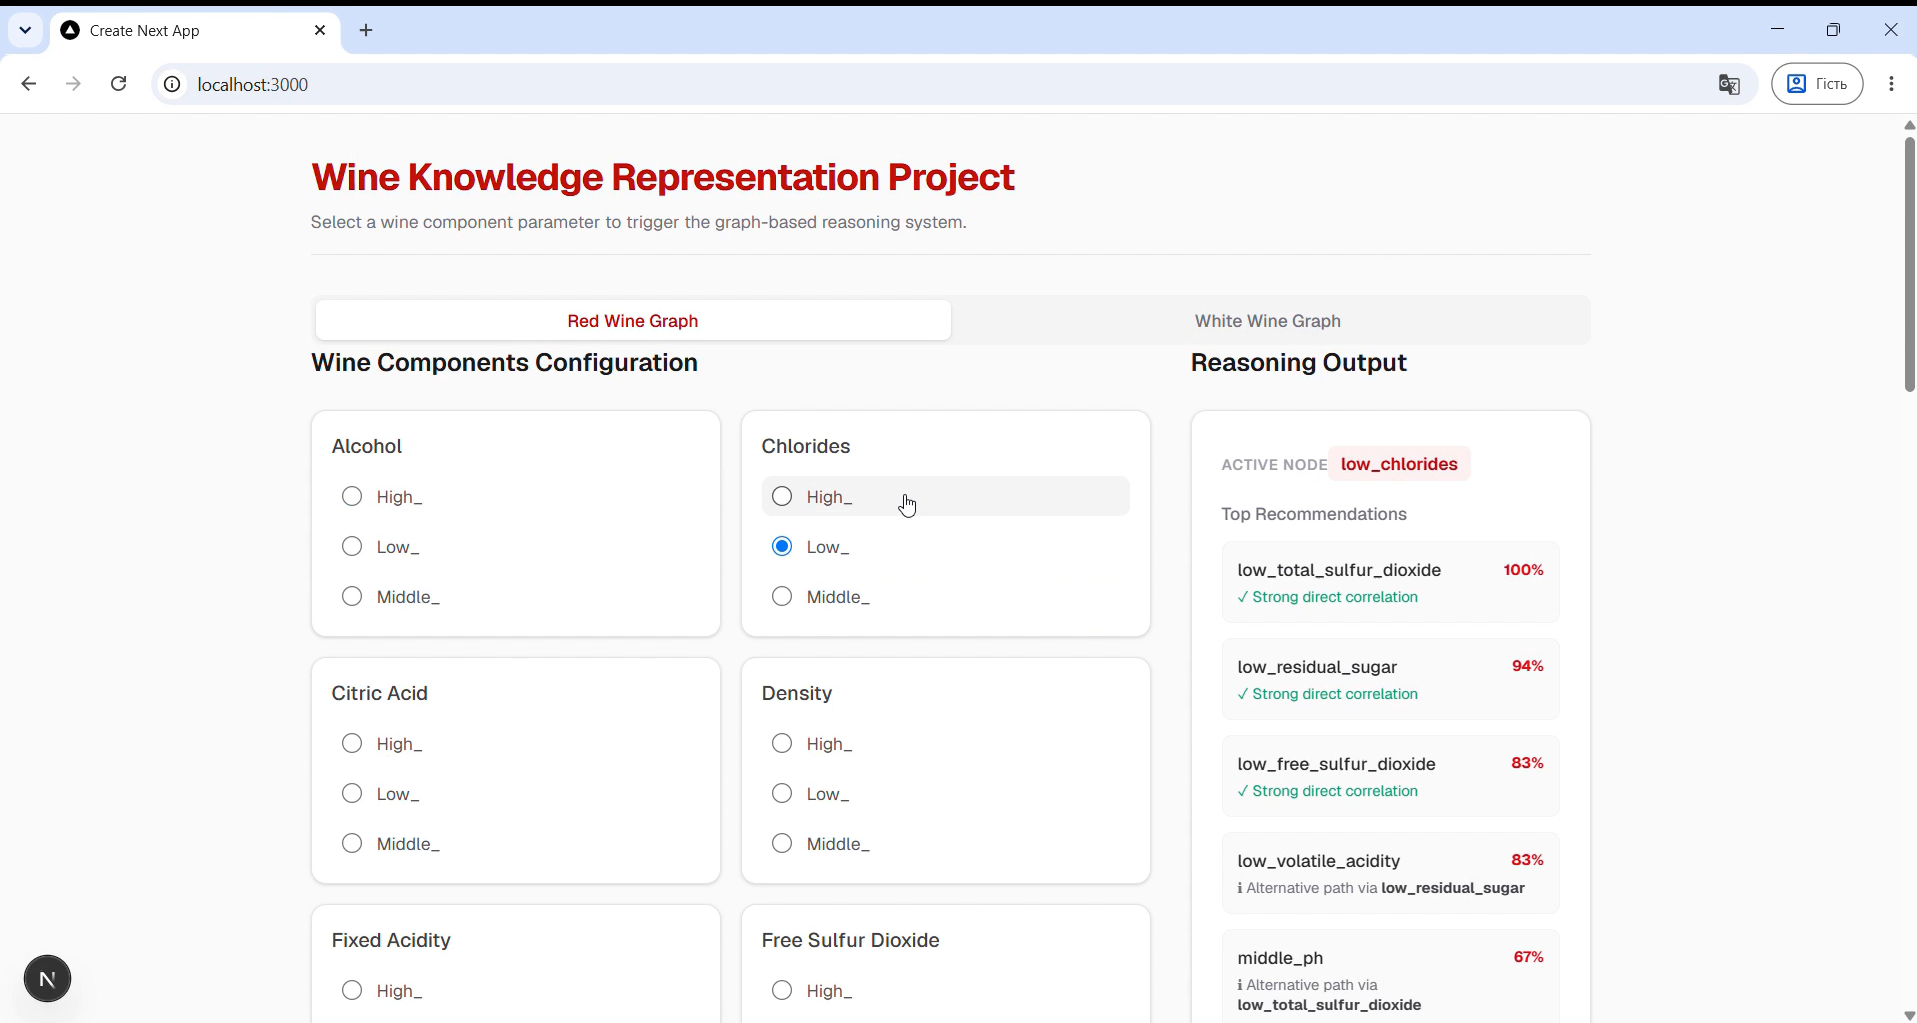
\includegraphics[width=\textwidth]{../imgs/screenshot.png}
	\caption{The same query in the web app: choosing \texttt{low\_chlorides} shows the
	five recommendations of Table~\ref{tab:trace}, each marked direct or indirect.}
	\label{fig:ui}
	\end{figure}

	\FloatBarrier
	\subsection*{Discussion}
	\textbf{Strengths.} The knowledge is explicit and easy to read; every
	recommendation can be explained; and the same graph can be written as RDF
	triples.

	\noindent\textbf{Weaknesses.} Appearing together does not mean one causes the other, so
	the results are not real winemaking advice. Splitting each feature into three
	equal parts is sensitive to outliers, and keeping only the top wines
	(\texttt{quality == 8}) leaves few red-wine samples, so some links rest on small
	counts.

	\section*{Conclusion and future work}
	% (about 1 page)
	We built an expert system whose knowledge is represented explicitly as a typed
	semantic network of wine-component associations, and whose engine reasons over
	that knowledge to recommend complementary components and to infer indirect
	associations with explanations. This directly addresses the three research
	questions: measurements are turned into qualitative concepts (RQ1), those
	concepts and their associations are represented as a typed, self-describing graph
	(RQ2), and graph traversal both queries and extends that knowledge (RQ3).

	\textbf{Limitations and future work.}
	\begin{itemize}
		\item Right now the graph only stores that two states appear together, and
		only for the best wines.
		\item It could be made richer by also comparing the best wines against the
		bad ones, to see what really makes a wine good.
		\item A useful next step is to store the knowledge as RDF/OWL and query it
		with SPARQL, and to add an OWL reasoner -- a tool that can work out new facts
		on its own, instead of only walking the graph.
	\end{itemize}

	\section*{Declaration of generative AI use}
	During this work, the author used Claude Code \citep{claudecode2026}, an AI
	coding assistant by Anthropic, as a support tool. The author checked and edited
	all results and takes full responsibility for the content of this report and
	the software.

	\bibliographystyle{plainnat}
	\bibliography{literature.bib}

	\vspace{0.5cm}
	\hrule
	\vspace{0.3em}
	\hrule
	\vspace{0.5em}
	\begin{center}
		\textbf{Note:} Source code:
		\url{https://github.com/Myron5/Wine-Recommendations-System}
	\end{center}

\end{document}
